\documentclass{beamer}

 \usepackage[german]{babel}
 \usepackage[utf8]{inputenc}
 \usepackage{graphicx}
\usetheme{Antibes}

\setbeamercovered{transparent}
\beamertemplatenavigationsymbolsempty
\setbeamertemplate{footline}[frame number]
\title[Raspberry Pi ROS]{Raspberry Pi ROS}
\author{Denis Herdt, Almin Causevic}
\institute[I_HS Wgt-Rav]{Angewandte Informatik HS Weingarten-Ravensburg}
\date{\today}
%\logo{\pgfimage[width=2cm,height=2cm]{hulogo}}
%\titlegraphic{\includegraphics[width=2cm,height=2cm]{hulogo}}
\subject{Raspberry Pi ROS}

\begin{document}
\frame{\titlepage}

\begin{frame}
\centerline{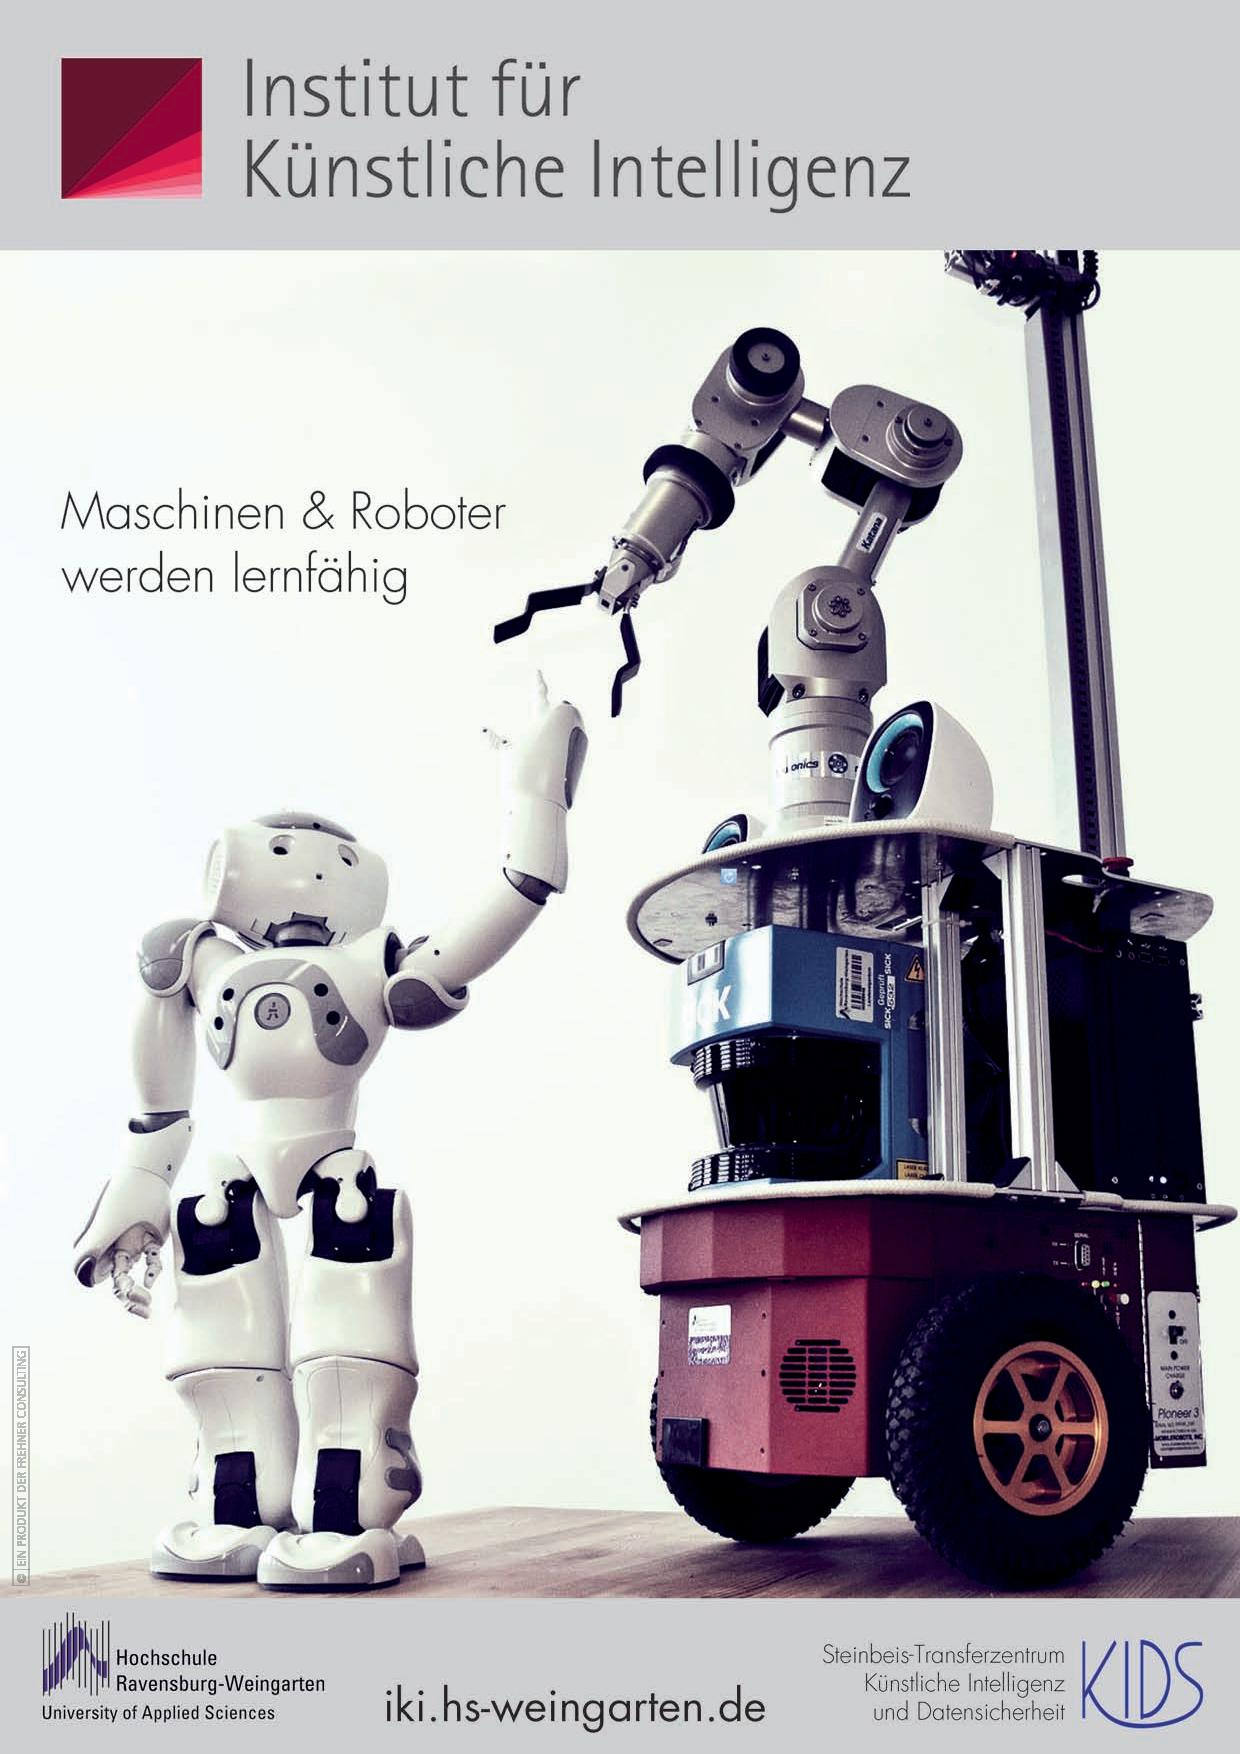
\includegraphics[width=7cm]{pics/iki.jpg}}
\end{frame}

\begin{frame}
{\bf Ablauf}
\begin{enumerate}
\item Projekte
\item Grundkonzepte
\item Installation
\item Netzwerk
\item Anwendung Volksbot
\end{enumerate}
\end{frame}

\begin{frame}
\centerline{
\includegraphics[width=9cm]{pics/ros5.png}}
\end{frame}

\begin{frame}
\centerline{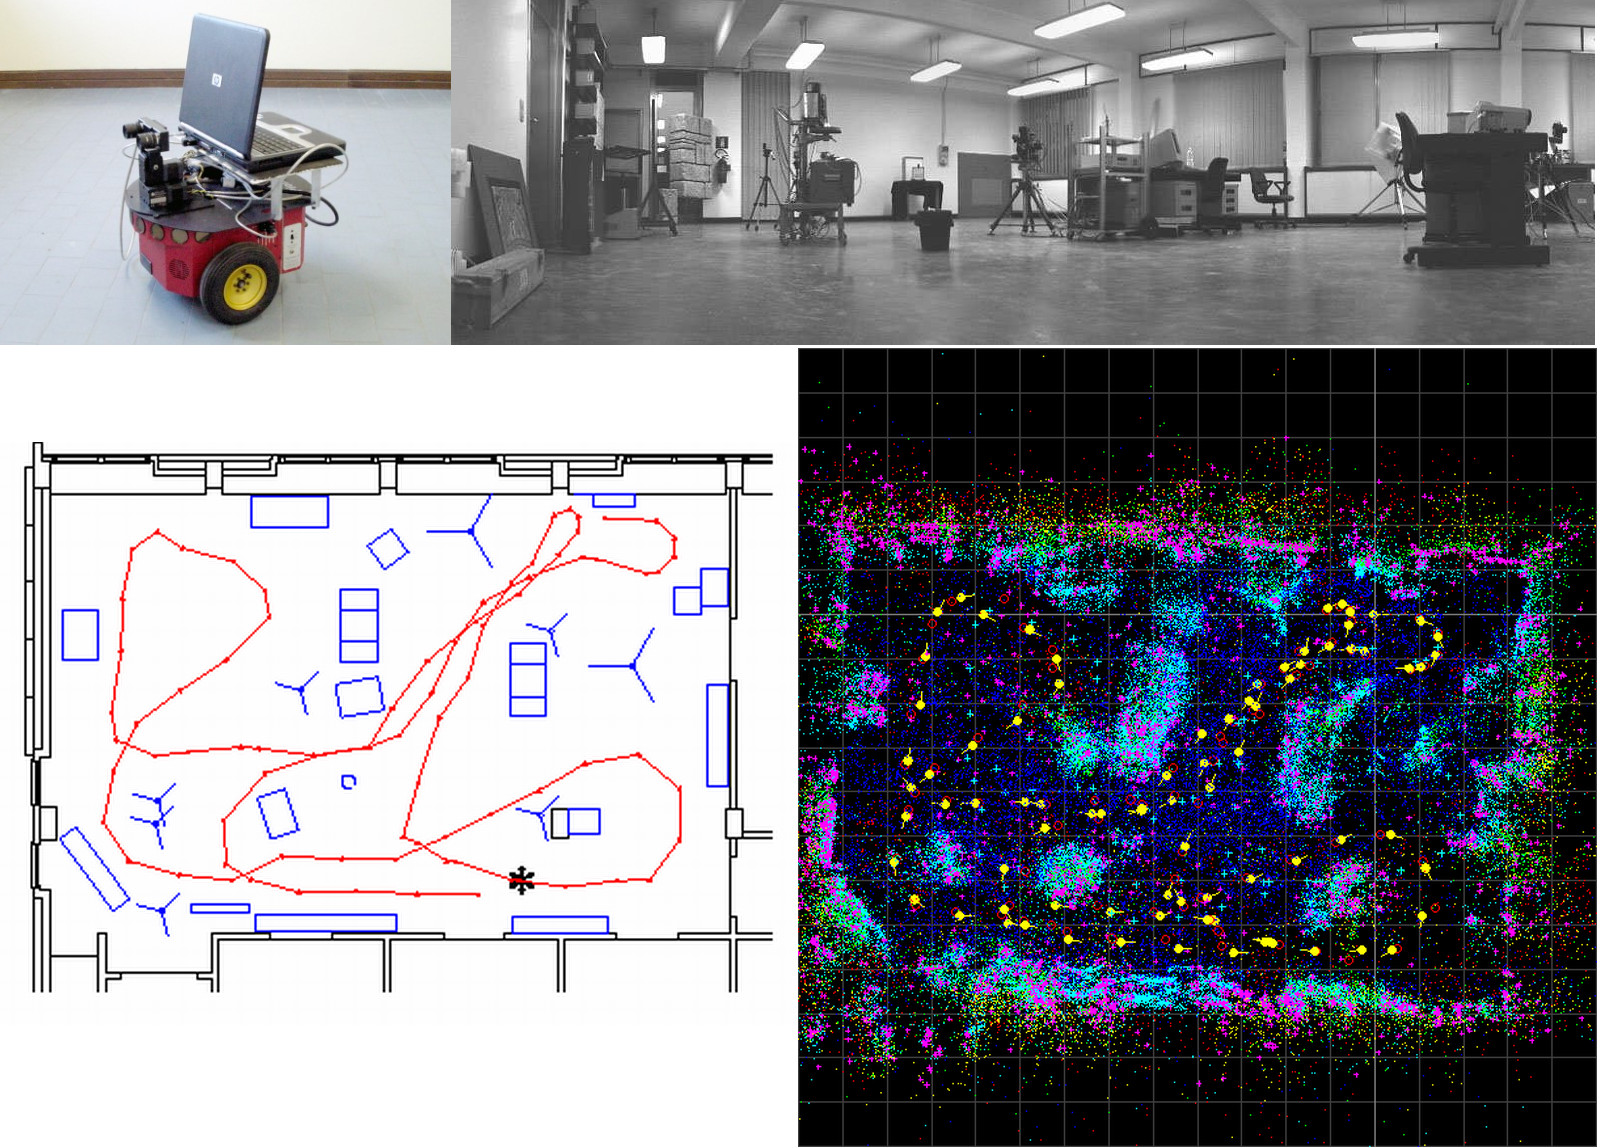
\includegraphics[width=9cm]{pics/slam.png}}
\end{frame}

\begin{frame}
\centerline{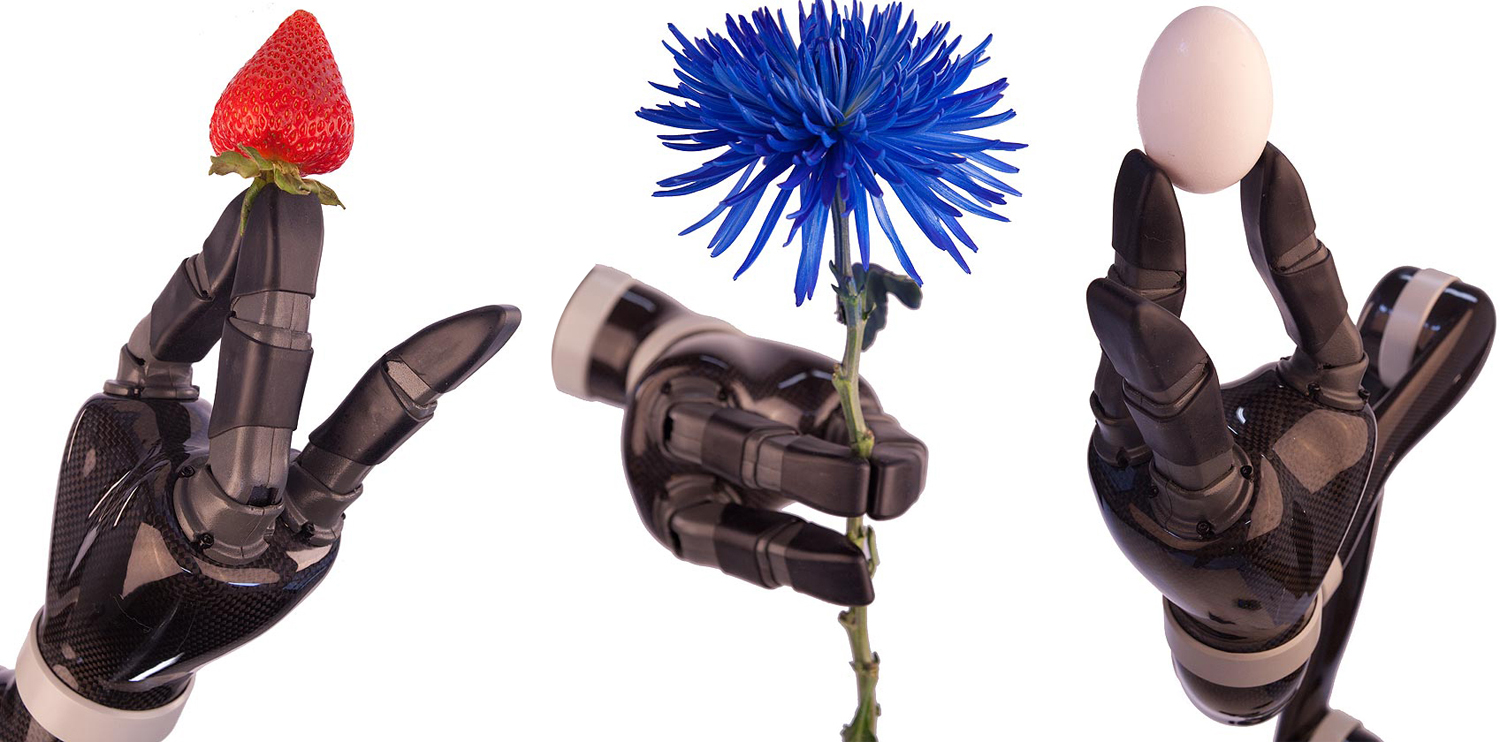
\includegraphics[width=9cm]{pics/jaco_arm.jpg}}
\end{frame}

\begin{frame}
Alternativen? \\
\parbox{5cm}{
\includegraphics[width=3cm]{pics/carmen.png}}
\parbox{5cm}{
\includegraphics[width=3cm]{pics/yarp.png}}
\parbox{5cm}{
\includegraphics[width=3cm]{pics/microsoft.jpg}}
\hspace{5cm}
\parbox{5cm}{
\includegraphics[width=3cm]{pics/orocos.jpg}}
\parbox{5cm}{
\includegraphics[width=3cm]{pics/orca.png}}
\end{frame}

\begin{frame}
\centerline{
\includegraphics[width=4cm]{pics/ros_equation1.png}}
\centerline{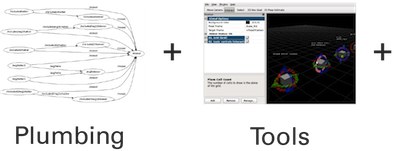
\includegraphics[width=6cm]{pics/ros_equation2.png}}
\centerline{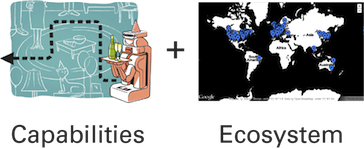
\includegraphics[width=6cm]{pics/ros_equation3.png}}
\end{frame}

\begin{frame}
\centerline{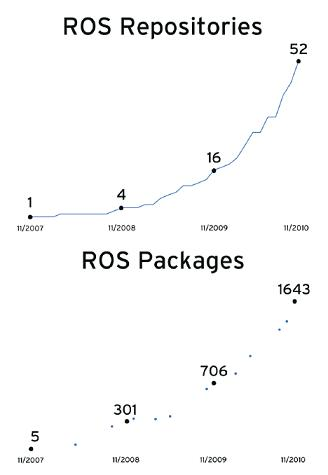
\includegraphics[width=6cm]{pics/ros_repos.jpg}}
\end{frame}


\begin{frame}
\parbox{5cm}{
\includegraphics[width=7cm]{pics/pilogo.png}}
%\huge %\hfill 
$\rightarrow$
\parbox{5cm}{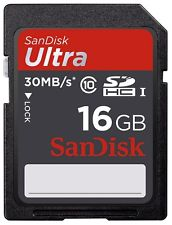
\includegraphics[width=3cm]{pics/sd.jpg}}
\end{frame}


\begin{frame}
\centerline{
\includegraphics[width=6cm]{pics/groovy.jpg}}
\end{frame}

\begin{frame}
{\bf ROS Installation}:
\begin{enumerate}
\item Source \\
$\rightarrow $ lehrreich \\
$\rightarrow $ zeitaufwendig \\
\item Binary \\
$\rightarrow $ triviale Installation \\
$\rightarrow $ wenige unterstütze packages \\
\end{enumerate}
\end{frame}

\begin{frame}
\centerline{
\includegraphics[width=4cm]{pics/goku.jpg}}
\vspace{2cm}
\centerline{{\bf \Huge FRAGEN?}}
\end{frame}

\end{document}
